Eine Velofahrerin fährt an einer Ampel los und beschleunigt in $t_1 = \tOneO$ gleichmässig auf $v_\mathrm{max} = \vMaxO$. Danach fährt sie $t_2 = \tTwoO$ lang mit konstanter Geschwindigkeit und bremst schliesslich in $t_3 = \tThreeO$ gleichmässig bis zum Stillstand ab.
\begin{center}
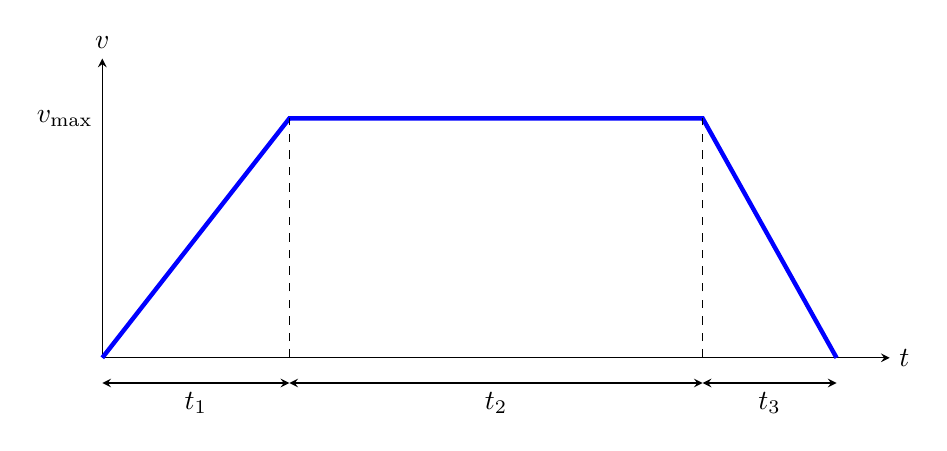
\begin{tikzpicture}[>=stealth, x=0.25cm, y=0.4cm]
 \draw[->] (0,0) -- (40,0) node[right] {$t$};
 \draw[->] (0,0) -- (0,9.5) node[above] {$v$};
 \draw[ultra thick, blue] (0,0) -- (9.5,7.6) -- (30.5,7.6) -- (37.3,0);
 \draw[dashed] (9.5,0) -- (9.5,7.6) (30.5,0) -- (30.5,7.6);
 \node[left] at (0,7.6) {$v_\mathrm{max}$};
 \draw[<->] (0,-0.8) -- (9.5,-0.8) node[midway, below] {$t_1$};
 \draw[<->] (9.5,-0.8) -- (30.5,-0.8) node[midway, below] {$t_2$};
 \draw[<->] (30.5,-0.8) -- (37.3,-0.8) node[midway, below] {$t_3$};
\end{tikzpicture}
\end{center}
\begin{abcliste}
\abc Welche Strecke legt sie insgesamt zurück?
\abc Wie gross ist ihre mittlere Geschwindigkeit?
\abc Zeichnen Sie die mittlere Geschwindigkeit in das $v(t)$-Diagramm ein und erklären Sie, was sie dort bedeutet.
\end{abcliste}
